\chapter{Bayesian estimation}\label{ch:bayes}

\begin{lstlisting}
nwergm [netname], edges [terms] estimate(bayes) [chains(#) burnin(#) iterations(#) thin(#)
    auxiterations(#) gamma(#) proposalvar(#) targetaccept(#) noadapt nodelayed dainflate(#)
    startvals(numlist) seed(#) priormean(numlist) priorvar(numlist) priorcov(matname)
    priordecay(# #) level(#) frame(name) nodraws]
\end{lstlisting}
With \texttt{estimate(bayes)} (synonym \texttt{method(bayes)}) \texttt{nwergm} returns the posterior distribution of the coefficients instead of a maximum likelihood estimate. It follows R's \texttt{Bergm::bergm()} (version 6.0.0; Caimo and Friel~\cite{caimo2011}). The normalising constant of the ERGM likelihood is not computed. The \emph{exchange algorithm} judges every proposal $\theta'$ with one auxiliary network $y'$ simulated from the model at $\theta'$: the acceptance ratio is $\exp\{(\theta-\theta')^\top(s(y')-s(y))\}\,\pi(\theta')/\pi(\theta)$ times the proposal ratio, where $s(y)$ are the observed statistics. The auxiliary network starts at the observed network and runs \opt{auxiterations()} (default 1000) Metropolis--Hastings steps in the compiled plugin, with the proposal of the fit.

\paragraph{The population of chains.} Several chains run together (\opt{chains()}, default $\max(2p,4)$ for $p$ coefficients). Chain $h$ moves to $\theta_h+\gamma(\theta_a-\theta_b)+\varepsilon$, where $\theta_a,\theta_b$ are two other chains and $\varepsilon\sim N(0,\sigma^2 I)$, $\sigma^2=$ \opt{proposalvar()} (adaptive direction sampling). The scale $\gamma$ starts at \opt{gamma()} (0.5) and adapts during the burn-in towards the acceptance rate \opt{targetaccept()} (0.25); \opt{noadapt} keeps it fixed. After the burn-in a Gaussian surrogate of the posterior, fitted to the second half of the burn-in with its covariance inflated by \opt{dainflate()}, rejects unpromising proposals before the auxiliary simulation is run (delayed acceptance, \opt{nodelayed} switches it off; it needs a burn-in of at least 10). The starting population is scattered around the pseudolikelihood estimate. The chains run one after another in one process.

\paragraph{Priors.} The prior is multivariate normal: mean \opt{priormean()} (default 0), variances \opt{priorvar()} (default 100) or a full covariance matrix \opt{priorcov()}. A free decay parameter of a curved term such as \texttt{gwesp(\#, free)} is sampled on the log scale with a log-normal prior, \opt{priordecay(}$\mu$ $\sigma$\opt{)} (default $\log 0.5$ and 0.75). Coefficients fixed by \opt{offset()} are held at their value.

\paragraph{Output.} The table gives the posterior mean, standard deviation, median, equal-tailed credible interval, the effective sample size (ESS, as \texttt{coda}'s \texttt{effectiveSize()}, summed over the chains) and the Gelman--Rubin statistic. \texttt{e(b)} is the posterior mean, \texttt{e(V)} the posterior covariance matrix, and \texttt{e(median)}, \texttt{e(sd)}, \texttt{e(ci)}, \texttt{e(ess)}, \texttt{e(rhat)}, \texttt{e(accept\_rate)} and \texttt{e(accept\_chains)} the other summaries. The draws are in the frame \texttt{nwergm\_bayes\_draws} (variables \texttt{b1}, \texttt{b2}, \dots\ in the order of the table, \texttt{chain}, \texttt{iter}).

\paragraph{Postestimation.} \texttt{estat mcmcdiag} shows ESS, Monte Carlo standard error, R-hat, the Geweke $z$, the autocorrelation and the acceptance rate by chain; with \opt{plot} trace and density plots (options \opt{name()}, \opt{saving()}, \opt{export()} and graph options as for \texttt{estat mcmcdiag} after a Monte Carlo fit, Section~\ref{sec:mcmcdiag}). \texttt{estat posterior} summarises the draws, saves them to a data set (\opt{saving()}, with \opt{replace}) and plots them (\opt{plot(trace|density|both)}, for the coefficients named in \opt{pars()}; Figure~\ref{fig:posterior}); because \opt{saving()} is the file of the draws, the graph is saved with \opt{gsaving(\emph{filename})} as a \texttt{.gph} file, exported with \opt{export(\emph{filename} [, \emph{options}])} (the options of \texttt{graph export}), and further graph options such as \opt{title()} go to \texttt{graph combine}; \opt{name()}, \opt{gsaving()}, \opt{export()} and graph options need \opt{plot()} (return code 198 otherwise), and the plot needs the core version~3.29.0 or later. \texttt{estat gof} becomes a posterior predictive check: it simulates networks at draws from the posterior (burn-in 10000 steps per network by default). \texttt{estat ic} is not available.

\begin{figure}[ht]\centering
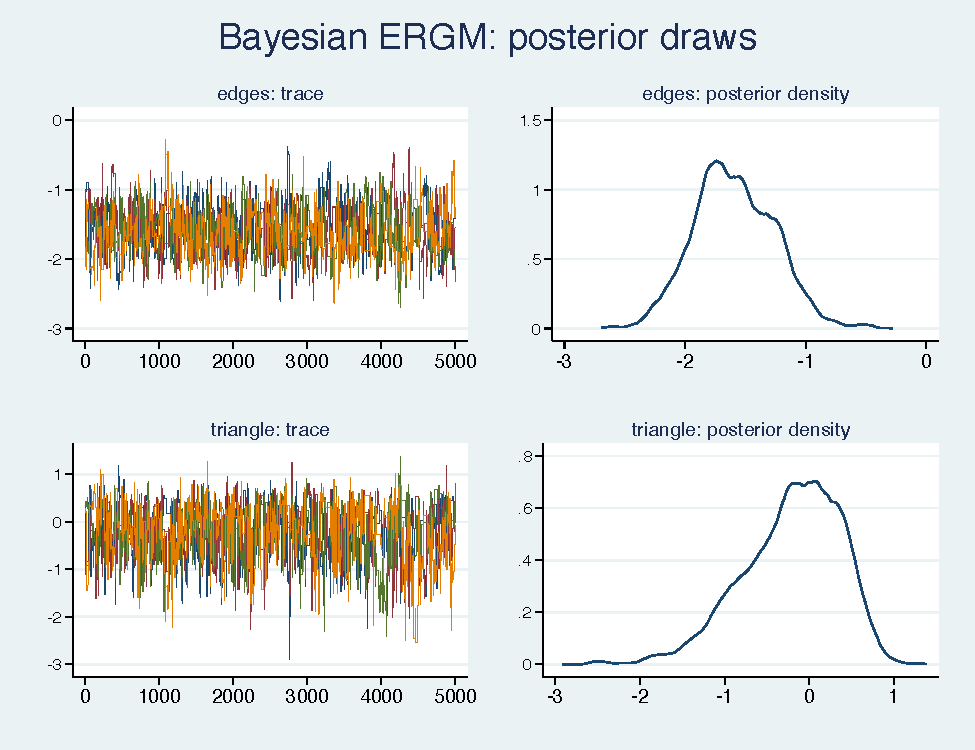
\includegraphics[width=0.85\textwidth]{fig/posterior.pdf}
\caption{\texttt{estat posterior, plot(both)} for the Florentine marriage network with \texttt{edges} and \texttt{triangle}, \opt{iterations(5000)} and \opt{burnin(2000)}: trace (left; one line per chain) and kernel density (right) of the draws of each coefficient.}\label{fig:posterior}
\end{figure}

\paragraph{Not available.} \opt{operators()}, \opt{constraints()}, \opt{obsconstraints()}, \opt{structural()}, \opt{fixdensity}, \opt{logstat()}, \opt{expstat()}, \opt{init()}, \opt{mainmethod()}, \opt{nonative} and networks with missing dyads are refused with \texttt{estimate(bayes)}.

\paragraph{Agreement with Bergm.} For a dyad-independent model the posterior can be computed by numerical integration; the sampler reproduces it (edges and a \texttt{nodematch} term on a wealth indicator of the Florentine families: means to two decimals, standard deviations within a few per cent). For the Florentine marriage network with \texttt{edges} and \texttt{triangle} the posterior means ($-1.60$ and $-0.2$) and standard deviations (0.33 and 0.58) agree with Bergm within Monte Carlo error, and for edges and a free-decay \texttt{gwesp} the decay has posterior mean 0.60 in both. The acceptance rates are 0.16--0.28 (Bergm 0.18--0.27). The compiled sampler is about six to eight times faster than Bergm in R on one core.
